\subsection{Commissioning \& Testing} \label{sec:hardware_testing}

After assembling each board, it is individually tested using the same testing procedure:

\begin{enumerate}
    \item Verify current consumption is within safe limits
    \item Attach testing harness to external connector
    \item Execute test software on test device and verify inputs \& outputs
\end{enumerate}

This chapter gives an overview of each individual step.

\paragraph*{Smoke testing}

The first step of the testing procedure is to verify the \ac{dut} is electrically sound by connecting only its power supply and ground lines. Both are connected to a power supply with a constant voltage and a current limit. The current limit is set to 3 times the estimated current draw. This estimated current draw is calculated by summing up the maximum current draw given in the datasheet of all components. The test is considered successful if the current limit is not reached. All boards passed the smoke test without issues or modifications.

\paragraph*{Testing harness}

After the electrical soundness of a board is verified, a temporary testing harness is attached. Since creating custom testing harness hardware for each type of board causes significant effort, instead, multiple individual wires are connected between the \ac{dut} and the test device. For this project, an ``Arduino MEGA'' is used. It is chosen because it was at hand and exposes more than 40 digital IO pins, as well as the previous experience of the author with the board. It is compatible with the \SI{5}{\volt} logic used for all modules and is programmable via USB. It also supports the widely used "Arduino" framework, which speeds up development and deployment of the testing code significantly. The board can be seen in \autoref{fig:arduino_mega}. \autoref{fig:register_under_test} shows a register \ac{pcb} with its testing harness attached.

\begin{figure}[H]
    \centering
    \begin{subfigure}[b]{0.49\textwidth}
        \centering
        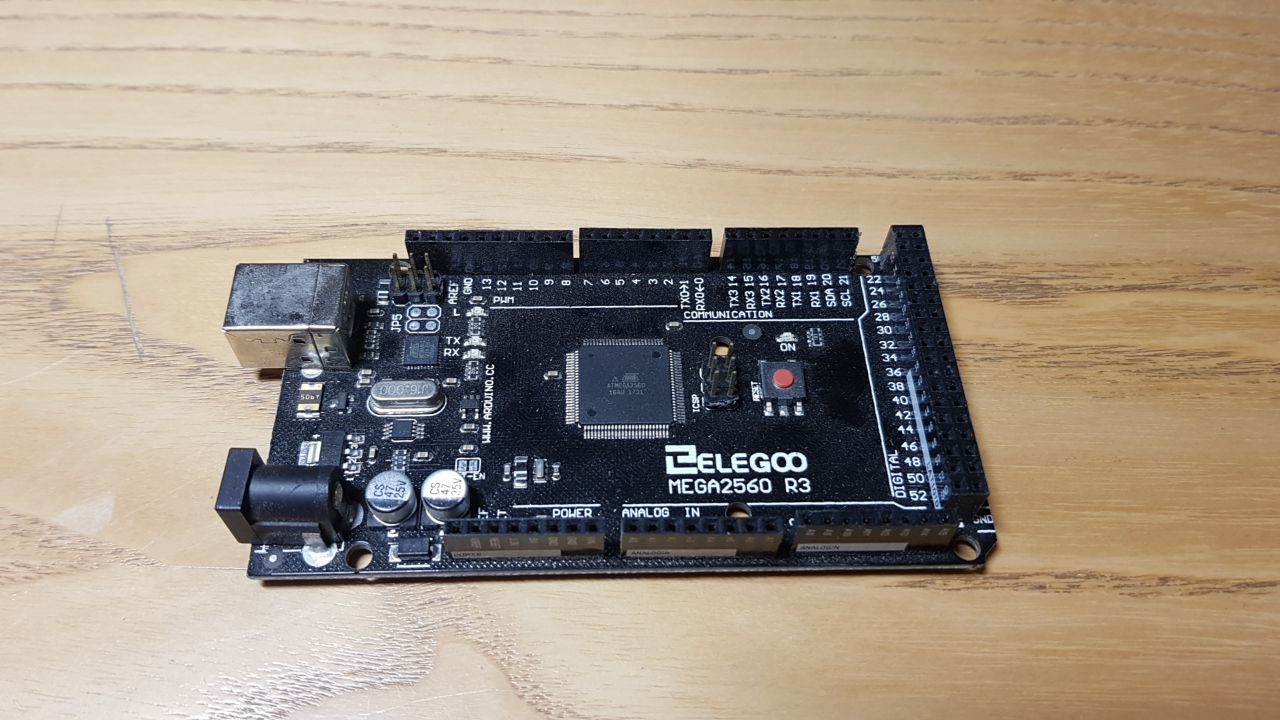
\includegraphics[height=1.5\textwidth]{images/arduino_mega.jpg} % Replace with your image file
        \caption[Arduino MEGA]{Arduino MEGA clone development board (compatible with Arduino)}
        \label{fig:arduino_mega}
    \end{subfigure}
    \hfill % Adds spacing between subfigures
    \begin{subfigure}[b]{0.49\textwidth}
        \centering
        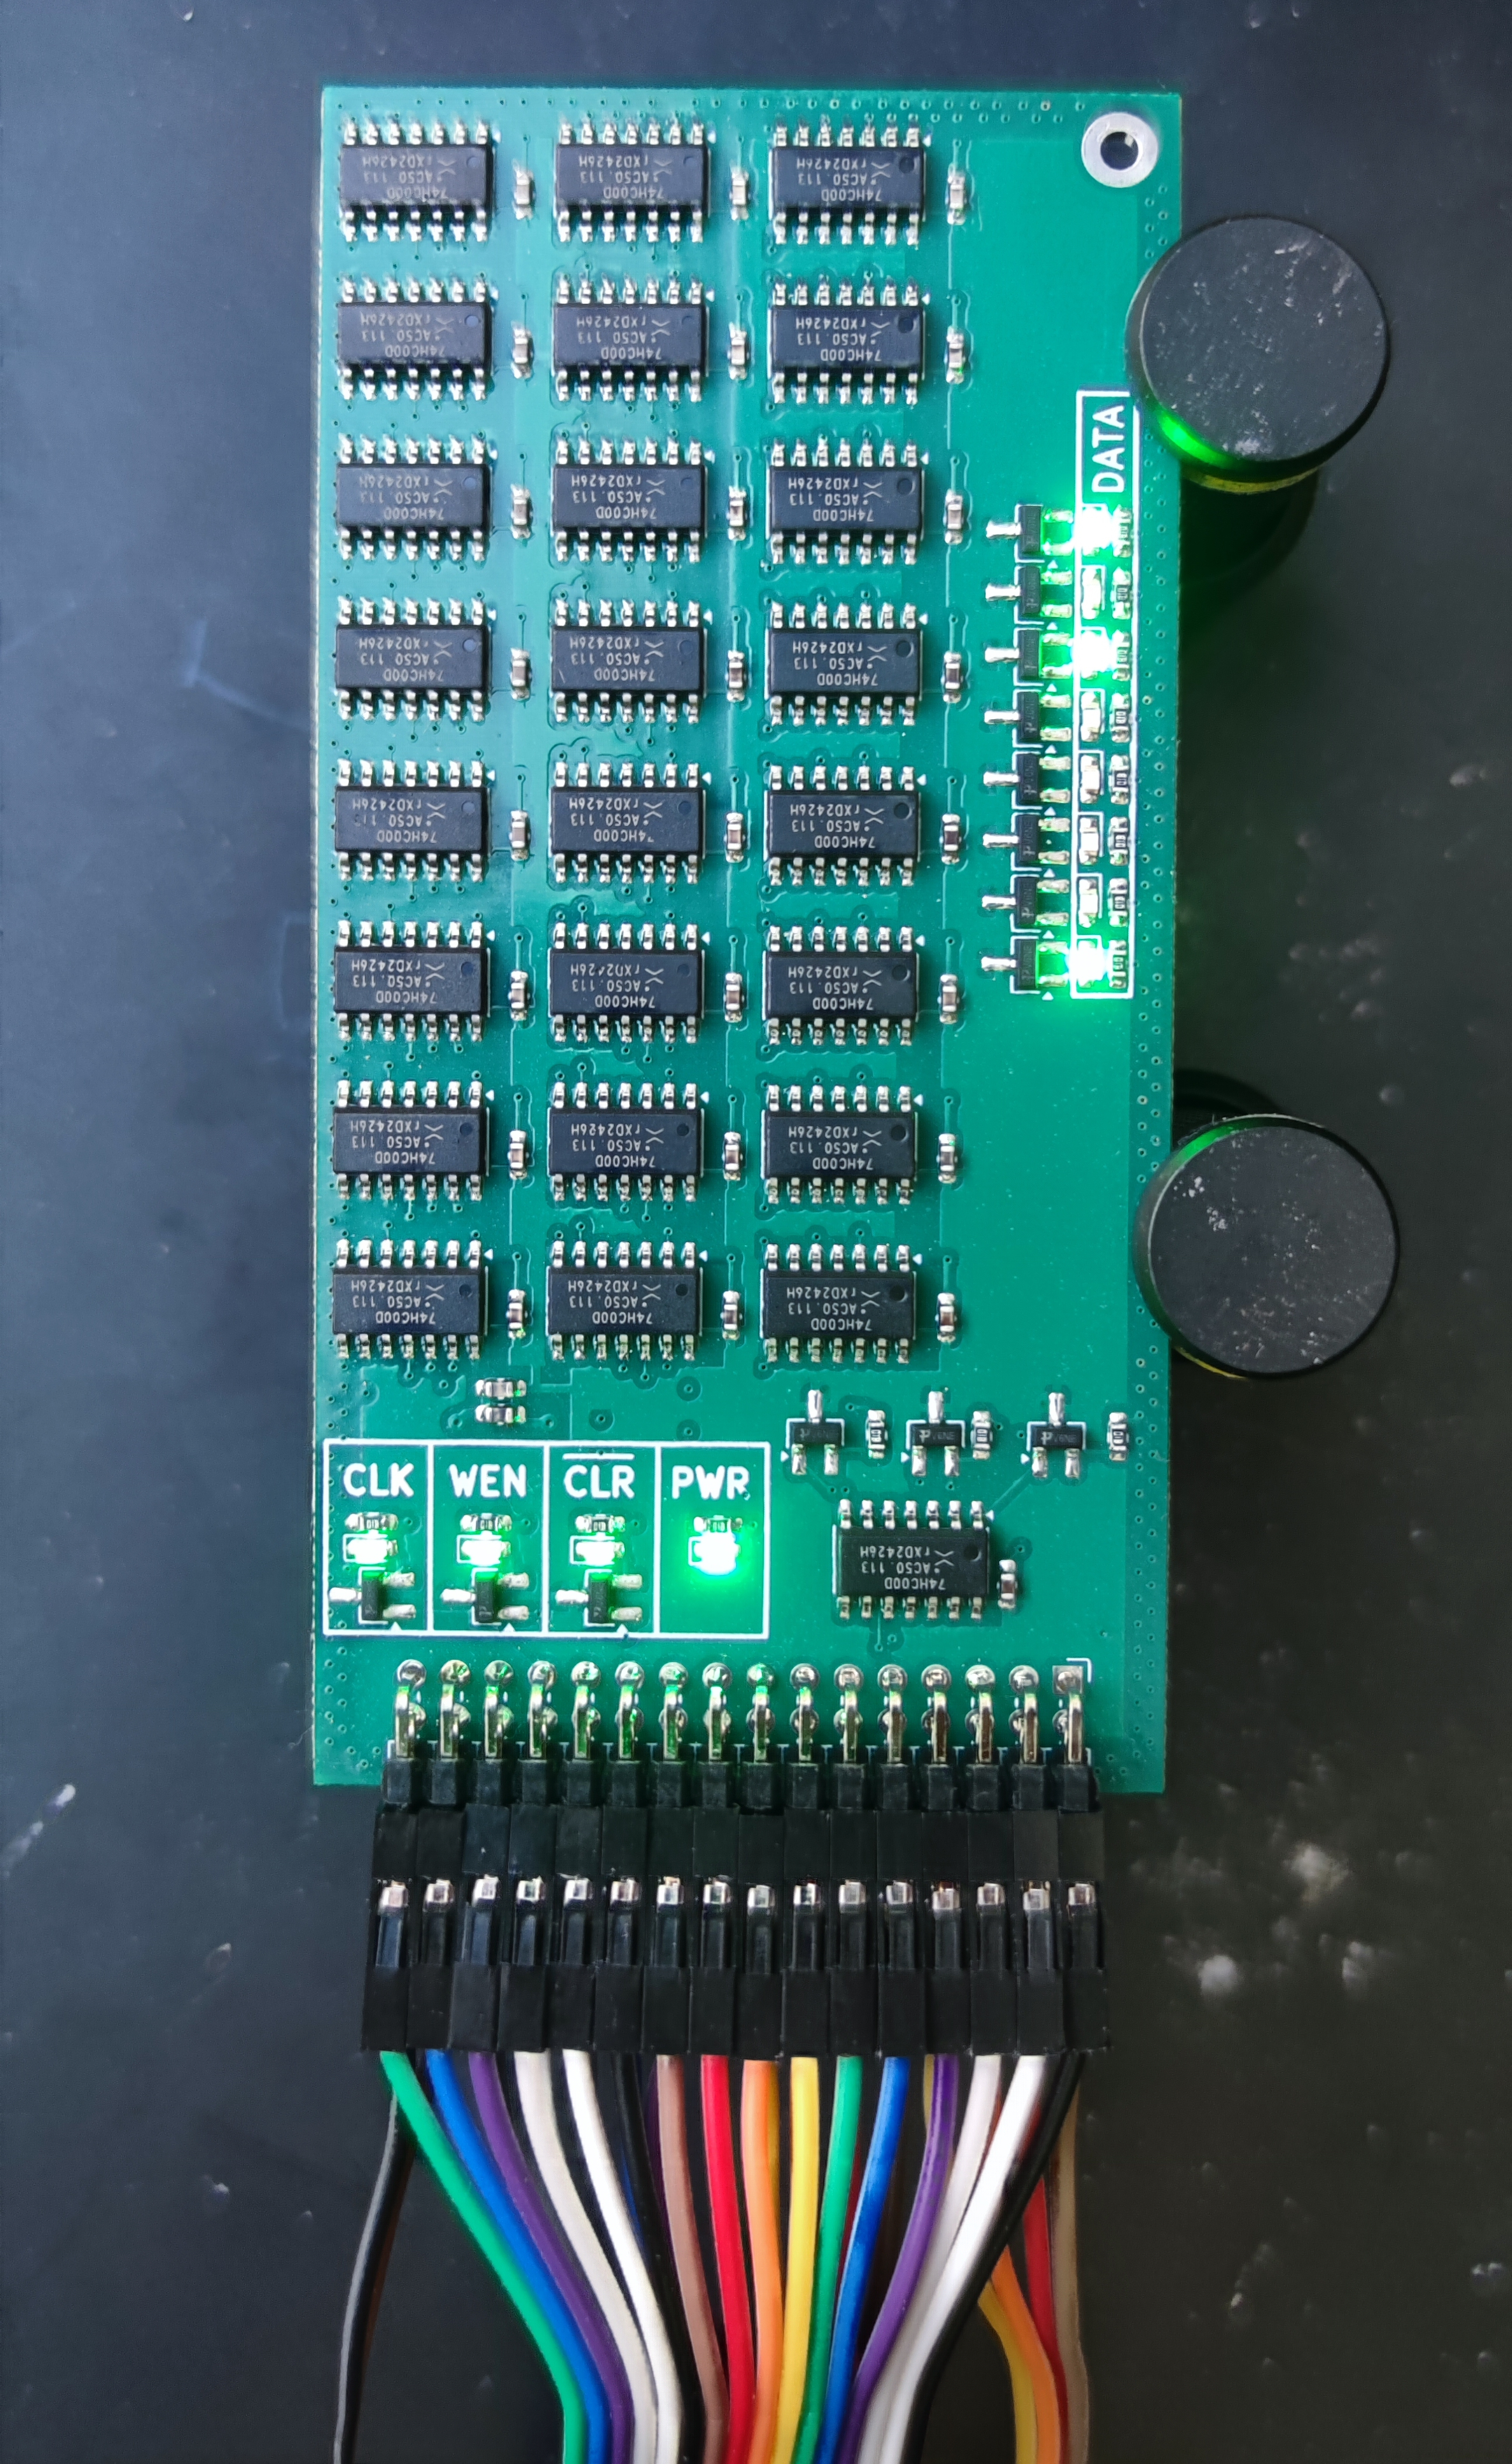
\includegraphics[height=1.5\textwidth]{images/register_in_test_jig.jpg} % Replace with your image file
        \caption{Register \ac{pcb} with attached testing harness}
        \label{fig:register_under_test}
    \end{subfigure}
    \caption[Test hardware]{Hardware used for testing individual modules}
    \label{fig:execution_models}
\end{figure}

\paragraph*{Testing software}

Each type of \ac{pcb} has its own set of testing procedures that are executed on the ATMega. This software mostly uses digital reading and writing on the \ac{io} pins of the ATMega, which then causes the tate of the \ac{dut} to change. This allows highly customisable testing. Due to the finite number of inputs and outputs of each module, it is feasible to exhaustively test many of them. For example, as the \ac{alu} operates on two 8 bit operands with 8 different operations, its input space contains only $2^{24} = 16777216$ states. At the time of writing, after applying the inputs, a delay of \SI{100}{\micro\second} is used to allow all signals to propagate through the device and allow its outputs to settle. With this delay, 10000 different states can be tested per second. This in turn allows exhaustive testing of the entire input state space in $\frac{2^{24}}{\SI{10000}{\hertz}} \approx \SI{1677.7}{\second} \approx \SI{28}{\minute}$.

\paragraph*{Results}

Due to time constraints, only the \ac{alu}, registers and register fabric are able to be tested. They perform as expected, except for the zero flag output of the \ac{alu}. It behaves identical to the overflow flag output. This is narrowed down to a via accidentally puncturing a trace carrying the overflow signal. This was not caught by KiCADs electrical rule checker tool for an unknown reason. This error is already corrected in the design files but has not been manufactured at the time of writing.
